\documentclass[conference]{IEEEtran}

\sloppy

%\pdfpagewidth=8.5in
%\pdfpageheight=11in


\usepackage{graphicx}
\usepackage{epstopdf}
\usepackage{subfigure}
\usepackage{wrapfig}
\usepackage{caption}
%\usepackage{subcaption}
%\usepackage{subfig}
\usepackage{amsmath}
\usepackage{xspace}
\usepackage{authblk}

\graphicspath{ {../fig/} }

% enable/disable margin comments
\newif\ifcomments
%\commentsfalse
\commentstrue

%\pagestyle{headings}

\begin{document}

\title{FLUX: A Next-Generation Resource Management Framework for Large HPC Centers}
\author{Dong H. Ahn, Jim Garlick, Mark Grondona, Don Lipari, Becky Springmeyer, \\
        Martin Schulz}
\affil{Lawrence Livermore National Laboratory, Computation Directorate, \\
        Livermore, CA 94550, \\
        \{ahn1,garlick,grondona1,lipari1,springme,schulzm\}@llnl.gov}

\date{}
\maketitle


\newcommand{\flux}{Flux}
\newcommand{\zMQ}{\O{}MQ}


\begin{abstract}
Resource and job management software is crucial 
to High Performance Computing (HPC) for efficient application execution. 
However, current systems and approaches can no longer keep up with the challenges HPC are facing
%centers are faced with major 
%resource and job management challenges that stem from 
due to
ever-increasing system scales, resource and workload 
diversity, interplays between various resources 
(e.g., between compute clusters and a global 
file system), and complexity of resource constraints 
such as strict power budgeting. 
%In this paper, we 
%argue for a new resource and job management paradigm 
%that can effectively address these emerging challenges
%under one common software framework.
To address this gap,
we propose \flux, an extensible job and resource management framework 
specifically designed to deal with the requirements of next generation HPC centers.
%
%that can embody this new paradigm
%in a simple, extensible, distributed, and autonomous fashion.
\flux targets an entire computing facility as one common pool
of diverse sets of resources enabling the it to accommodate
site-wide constraints (e.g., for power limits), yet its scalable
and distributed design still  
offers scalable and effective scheduling strategies. 
%as well as flexible accommodation of site-wide constraints.
%Further, its run-time system is designed to support the 
%new paradigm, providing high scalability and user 
%productivity. 
This paper details the design of \flux and describes and evaluates
our initial 
prototyping effort of the key run-time components. 
Our results show that our run-time prototype 
provides strong and predictable scalability. 
\end{abstract}

%\keywords{{resource management, communication framework, run-time,
%key value store, scalable process management services.}}
\section{Introduction}

Resource and job management software (RJMS) is critical
for high performance computing (HPC).
It is the centerpiece that enables efficient
execution of HPC applications while providing
the computing facility with the main means
to maximize the utilization of its diverse array 
of computing resources~\cite{GeorgiouThesis}.
However, several growing trends make even
best-in-breed RJMS systems increasingly
ineffective in dealing with the diversity and size 
of resources fielded for HPC centers.
As numbers and types of compute resources
continue to grow, the key management challenges 
traditionally associated with only a few individual 
extreme-scale machines~\cite{sequoia,titan} 
quickly permeate through all computing resources 
(e.g., commodity Linux clusters) 
sited at a center. 
RJMS now must provide all of the resources at the center
with extreme scalability, low noise, fault tolerance, 
and heterogeneity management delivered 
within increasingly stricter power bounds.

In addition, greater difficulties in code development
on larger systems impose increasingly challenging 
requirements on the RJMS. Without adequate
RJMS support, debugging, tuning, testing, and verification
of applications have become too difficult and 
time-consuming for end-users~\cite{STAT,SPINDLE,PRUNER,SCR,launchmon}.
Next-generation code development environments
require the RJMS to provide effective mechanisms
to ease this user burden with features that support 
the reproducible results of program execution,
provide accurate correlations between user-level errors
and system-level events,
and facilitate integration and development 
of a rich set of scalable tools.
Unless the RJMS can effectively
address these shortcomings, HPC centers and their users 
can suffer significant productivity losses.

The traditional resource and job management paradigm
for large HPC centers organize the resources sited
at a center in a static and flat hierarchy. Typically, it 
runs an RJMS instance~\cite{Jette02slurm} to manage an individual cluster
and those instances are connected together by 
grid software~\cite{MOAB,PSBPro,LSF}.
While simple, a greater interplay 
among various classes of clusters across the center
are already making this paradigm increasingly 
inflexible and ineffective. 
For example, the current paradigm cannot effectively
schedule applications that utilize site-wide shared 
resources such as file systems. 
Without scheduling a file I/O-intensive job 
to both compute resources and the dependent storage 
hierarchy, overlapping I/O bursts coming from only a few
unrelated jobs can randomly disrupt the entire center~\cite{SCR,SPINDLE}. 
In addition, with a flat hierarchy, imposing complex 
resource constraints at various levels at the center
is becoming increasingly difficult. 
%Avoiding any significant site-wide bottleneck
%requires the RJMS to schedule the job to all dependent
%resources that often span the boundaries 
%of a single cluster.


In this paper, we argue for a new paradigm that can
effectively address the resource and job management 
challenges that large HPC centers are increasingly facing.
We argue that the new paradigm must increase its purview 
to manage resources across the entire center under
one common RJMS framework, and 
be able to (co-)schedule jobs to various types of resources.
We argue that the new paradigm must facilitate 
scheduler parallelism~\cite{Omega,Mesos}. Further, it must
provide the parallelism through hierarchical, multilevel 
scheduling schemes with support for arbitrary numbers of levels, and 
be capable of specializing each level.

It will be a long journey to fully implement this new paradigm. 
But we have made a few significant steps to embody the paradigm:
we started to develop an open-source RJMS framework, \flux,
and to explore its run-time core components.
Thus, this paper also presents our early explorations
of two core run-time elements: 
communication framework termed the Comms Message Broker (CMB)
and workload run-time services for efficient, interoperable
launching and organizing of the distributed processes.
CMB represents a novel back-bone overlay network for \flux,
which can replace all the redundant and independent
daemon infrastructures that currently exist in a typical cluster.

This paper makes the following contributions:
\begin{itemize}
\item{Emerging resource and job management challenges that demand a new paradigm for large HPC centers;}
\item{The design concept of \flux\ emboding this paradigm;}
\item{Core run-time components of \flux\ as enablers of this paradigm;}
\end{itemize}

The results of our performance evaluation 
and performance model show that KVS and CMB provide 
strong and predictable scaling properties.
%Further, our case study on integrating various key run-time software software
%programs indicate that \flux's run-time elements 
%provide these programs with 
%easy integration and interoperability.
These results continue to guide our design choices
as we progressively realize our vision. 


\section{A New Management Paradigm for HPC}
\label{label:paradigm}
HPC centers typically provide a wide range of 
platforms on which scientific applications perform
computations.
The RJMS system is responsible for efficiently delivering 
compute cycles of these platforms
to multiple users who must submit jobs to run their applications. 
Thus, the RJMS matches the users' job request with the available 
resources and provides efficient functions 
for building, submitting, launching and executing, 
and monitoring jobs~\cite{GeorgiouThesis}. 
Typically, an HPC center runs an RJMS instance~\cite{Jette02slurm} 
to manage and schedule an individual system (e.g., cluster) and 
additionally employs separate grid software to tie 
these instances together. 

However, several growing trends present major challenges 
to this current management paradigm. 
First, systems sited at one center are growing larger 
and types of resources are becoming increasingly diverse~\cite{GeorgiouThesis}. 
%The RJMS must now provide  
%extreme scalability, low
%noise, fault tolerance, and heterogeneity management
%to most of the resources sited across the entire center. 
Second, interplays between 
various classes of resources
(e.g., between compute clusters and a global file system)
are becoming more complicated and disruptive~\cite{SCR,SPINDLE}. 
Third, resource constraints are also becoming increasingly
complex in a multidimensional, dynamic, and hierarchical fashion~\cite{power-overprovision}
(e.g., dynamic power capping at the level of systems, compute racks, and/or nodes).
Further, the need for code-development tools and their requirements on tool launching and job access
impose challenging requirements on the RJMS~\cite{STAT,SPINDLE,PRUNER,SCR,launchmon}.
Finally, the workloads themselves are becoming 
diverse, dynamic, and large, and are moving away from individual monolithic jobs. Instead,
ensembles of jobs, e.g., for Uncertainty Quantification 
%DONG: We need a refernece to use Scalebriging Application
or Scalebriding Applications, are becoming increasingly commonplace.

To address the issues effectively,
large HPC centers demand a new resource and job management paradigm.
The new paradigm must increase its purview and 
scalably manage resources across the entire center.
Perhaps more importantly, it must be implemented under one common 
RJMS framework so that its schedulers can make use of
its full resource representations.
Only this allows centers to (co-)schedule jobs 
effectively to various types of resources and to
provide much richer provenance on jobs (e.g., correlation between
a user-level error and other system activities). 
%A divide-and-conquer approach will enable the RJMS 
%to scale to the entire center. 
The new paradigm, however,
creates a series of challenges a new RJMS must overcome:

%It is important to note that all of these must 
%be enabled by one common RJMS framework. 
%The current paradigm of loosely coupling different software 
%(i.e., grid software with cluster-wide RJMS instances) 
%leads to a loss of important system knowledge
%needed for effective resource and job management and scheduling. 
%Different software employ distinct resource and
%job representations and key data are often lost in translation.
%Also, the single common framework can offer 
%common run-time commonents as a backbone of
%supporting hierarchical management of resources and jobs
%in a highly scalable, fault-tolerant, secure and customizable
%manner.

%We realize that embodying the new paradigm is non-trivial, as
%the following characterizes the challenges it must address.

\noindent{\em Challenge 1: Multidimensional Scaling --- } 
The new paradigm requires that the RJMS can impose
complex, multidimensional resource bounds at any scale, 
from the center-wide level, down to the level of individual processes,
and enable the most efficient execution and
scheduling of workloads within these bounds.
This imposes unprecedented scale challenges
in multiple dimensions,
%We generally characterize this challenge 
%as the {\em multidimensional scale} challenge. The challenges
% include
supporting extreme scalability, addressing noise as concurrency
increases, and managing a drastically increased amount of
run-time information that must be monitored, traced, and stored.
The new paradigm must efficiently handle increased scale in
numbers of resources as well as jobs and other dimensions 
of RJMS data.

\noindent{\em Challenge 2: Diverse workloads --- }
HPC applications are known to have disparate performance 
limiting factors. This requires
the new paradigm to have a rich resource model, including
the 
%This includes a 
representation for diverse
types of resources such as file systems, networks, visualization
hardware, and heterogeneous compute engines.
With a richer resource model, the RJMS will be capable of imposing
complex, multidimensional resource bounds, as opposed to the
simplistic traditional resource model that is fundamentally based on a
flat list of nodes, and allowing it to 
%With the ability to model sophisticated resource relationships,
%the new paradigm will be able to schedule and
allocate resources tailored to the disparate limiting
factors of HPC applications.  

\noindent{\em Challenge 3: Dynamic Workloads --- }
Resource allocations
must be elastic, i.e., resource allocations must be able to grow and shrink
dynamically. This is necessary to support HPC applications with different
phases with disparate performance-limiting factors.
Different resource types have different
elastic properties 
(e.g., power is a much more elastic resource than compute nodes)
restricting decision points and allocation granularity.
%HPC applications and their programming models are
%becoming increasingly dynamic with different multi-resource requirements
%at different phases. 
One consequence of this is that the RJMS must 
support multiple levels of elasticity 
as a function of dynamically changing performance limiters
as well as their limiting resource types---e.g., 
rigid vs. moldable vs. malleable scheduling~\cite{Convergence} 
against different workload and resource types.

\noindent{\em Challenge 4: Productivity --- }
The new paradigm must address increasing complexities
in code development and system administration by facilitating
the creation of more effective diagnostic and analysis tools.
For example, it must provide basic, scalable monitoring and communication
primitives at the job level that can be leveraged by tools.
It will encourage a richer, stronger tool ecosystem.
% where
%these basic but non-trivial capabilities need not be recreated
%from scratch in every tool, reducing development costs.
Better tools will lead to higher productivity for all
stakeholders, including end users.
%We characterize this design challenge as the {\em productivity challenge}.

\noindent{\em System Challenges --- }
In addition to these main requirements that come from the user side
of the RJMS, we also face internal challenges that need to be hidden
from the user. 
%We have considered additional challenges. 
For example, in a global model,
the risk of higher downtime costs arises. 
%in a more global model.
If the RJMS is inadequately designed, a downtime could negatively
impact the availability of a large portion of the center's
resources. Thus, it must be tolerant of hardware and software
faults and failures with no single point of failure and 
also support live software upgrades. 
Other challenges include security, integration risk, 
and backwards compatibility. 
%will be addressed in our future work.

%

This series of challenges strongly motivates 
a specific management and scheduling scheme:
the new RJMS must hierarchically and dynamically
manage and schedule the resources under one
common software framework. The divide-and-conquer
approach will then allow the RJMS to scale to massive
amounts of resources sited at a large center.  
%Undoubtedly, such a new paradigm will face unprecedented scaling challenges.
%in job scheduling. a RJMS 
%Thus, it 
Further, the hierarchical, multilevel job scheduling
will then facilitate scheduler parallelism~\cite{Omega,Mesos},
and this will allow the RJMS to scale to massive numbers
of jobs scheduled across the center.
In this scheme, higher-level schedulers
must allow a site to impose site-wide policies, contracts,
and constraints while lower-level schedulers should allow
efficient use of any subsets of resources in accordance with
workload types.
Finally, the RJMS must be capable of dynamically supporting
arbitrarily deep levels in this management and scheduler 
hierarchy with an ability to impose
different constraints at each level.



\section{Conceptual design of \flux}
\label{models}
Flux is the open-source RJMS framework we are actively
investigating to embody the new paradigm while
addressing the multitude of challenges described above.
This section describes some of its fundamental design
concepts.

\vspace{1ex}
\noindent{\em Unified Job Model: } In the traditional paradigm, 
a job is simply defined to be a resource allocation. 
But \flux\ unifies this notion with an independent 
RJMS instance. Because any \flux\ job has 
an independent resource and job management services,
it can recursively accept and schedule jobs and provide its own 
services to them. 
The RJMS instance must be delegated
the main responsibility of managing the resources allocated
to its job. But it must allow specialized service
plug-ins to be instantiated so that these resources
can be used differently than other resources.  
This model forms 
the foundation for a hierarchical,
multilevel resource management and job scheduling
with resource subset specialization.

\vspace{1ex}
\noindent{\em Job Hierarchy Model:} To scale the new paradigm 
to the entire HPC center, we must avoid a centralized approach. 
Instead, \flux\ employs a hierarchical resource management 
and job scheduling by forming a tree-based hierarchy of \flux\ jobs. 
Several guiding principles throughout the job hierarchy strike 
a balance between the management responsibility 
of a parent job and delegation and empowerment of a child job:

\begin{itemize}
\item{Parent bounding rule: the parent job grants 
and confines the resource allocation of all of its children.}

\item{Child empowerment rule: within the bound set 
by the parent, the child job is delegated the ownership 
of the allocation and becomes solely responsible 
for most efficient uses of the resources.}

\item{Parental consent rule: the child job asks 
its parent when it wants to grow or shrink the resource 
allocation, and it is up to the parent to grant the request.}
\end{itemize}

This model has many advantages for scalability of both
resource management and job scheduling. 
The independent and specialized \flux\ service instance
of a job becomes only responsible for managing its direct
child jobs, which would be only a small fraction of
the total number of jobs at the center. 
As sibling jobs run simultaneously, their independent
\flux\ instances will perform concurrent management services.

For example, for job scheduling, this model enables \flux\
to exploit scheduling parallelism~\cite{Omega,Mesos}.
A parent scheduler schedules at coarse granularity 
over a large collection of resources and leases different resource subsets 
to its children schedulers. 
At the same time, this will enable Flux to specialize the scheduling behaviors 
on subsets of resources without having to introduce a
complex global scheduling policy into the centralized, monolithic scheduler. 

In short, this model enforces the first principle 
of the new paradigm: imposing highly complex resource bounds 
to provide high operational efficiency 
at any level across the entire center, while enabling 
most efficient execution and scheduling of the workloads 
within these bounds. 
Further, this addresses 
many of the identified challenges in Section~\ref{label:paradigm} 
including the {\em multidimensional scale} and 
{\em diverse/dynamic workload} challenges. 

%\vspace{1ex}
\noindent{\em Generalized Resource Model:} In the traditional 
paradigm, compute resources are modeled primarily 
as a collection of compute nodes. But this is a simplistic perspective 
ill-suited for the new paradigm. Today's applications 
are diverse with disparate limiting performance factors 
beyond floating point computation. 
Further, computing centers are increasingly concerned 
about managing new resource types such as power 
and shared persistent storage. Our generalized resource
model addresses this need by providing an extensible
and flexible representation for resources
and their relationships.

%\vspace{1ex}
\noindent{\em Multilevel Resource Elasticity Model:} As our 
applications and their programming models are becoming 
increasingly dynamic, the new paradigm demands 
an elasticity model where an existing resource allocation 
can grow and shrink, depending on the current needs 
of applications and/or the HPC center. 
\flux\ supports the elasticity model within our job hierarchy 
framework above: a child job sends a grow or shrink request 
to its parent, which can go up the job hierarchy 
until all requisite constraints are known for this request. 
Also, combining this with the generalized resource model, 
the elasticity can be expressed for various resource including 
power consumption. Our elasticity model addresses 
the {\em dynamic workload} challenge.

%\vspace{1ex}
\noindent{\em Common Scalable Communication Infrastructure Model:} 
Our scalability strategy with respect to a large number 
of compute nodes is to provide a common scalable communication 
framework within each job. When a job is created, a secure, scalable 
overlay network with common communication service is established 
across its allocated nodes. Except for the root-level job, 
the existing communication session of the parent job assists 
the child job with rapid creation of its own session. 

A communication session is only aware of its parent 
and child and passes the limited set of control information 
through its communication channel. Thus, this model 
enables highly scalable communication within a job, while 
limiting communications between jobs, addressing 
both the {\em multidimensional scale} as well as security issues.
Further, this backbone per-job communication network 
supports well-known bootstrap interfaces 
for distributed programs including many MPI implementations 
as well as run-time tools. This provides tightly integrated support
for the development and use of scalable run-time tools, which 
can have a large impact on user productivity.

\section{\flux}


It is a serious undertaking 
to design the production version of a new 
RM framework that can realize our proposed conceptual models.
Thus, \flux\ team has engaged in a series of steps
meant to inform our design process. 
We began with a functional design including an
internal review with stakeholders including 
systems, run-time, and applications developers.
as well as run-time and applications level.
Subsequently, we initiated a prototyping phase for the \flux\ run-time.


%Then, this notion provided us with a concise 
%mechanism by which we can relate groups of processes
%to underlying resources (e.g., containing certain processes 
%to a set of resesources) as well as relate groups
%one another (e.g., synchronizing tool processes to 
%MPI processes). 
%
As part of the protyping exercise, we have developed a communication framework 
called the Communication Message Broker (CMB) 
as well as a scalable key value store (KVS) service.
They comprise essential scalable building blocks of our run-time system, 
and have allowed us to build various run-time services as well as
to port user-level run-time software programs to our prototype.
Further, we developed support for our concept of the lightweight 
job (LWJ) as a new way to organize distributed or parallel processes.
Using this notion, a wide range of run-time software
programs such as parallel programming models,
tools, and middleware can leverage our common run-time services 
to build upon \flux\ and eachother.

\ifcomments
\marginpar{\tiny BS: Do you want to now make a case for why KVS is going
to be an important building block?  Or just launch into the next
two sections on CMB and V'S?}
\marginpar{\tiny DA: I think I made a case. Let me know if not}
\fi

\subsection{Communication Message Broker}


A communication framework supports our hierarchical job model
by establishing a {\em comms session} to contain each \flux\ instance
and provide a foundation for the distributed components upon which
\flux\ will be built.
This framework enables secure, scalable communication
within a comms session, limits communication between sessions,
and allows new comms sessions to be created, resized, destroyed,
and monitored by existing ones in a parent-child relationship.

\begin{figure}
\vspace{-.5cm}
\centering
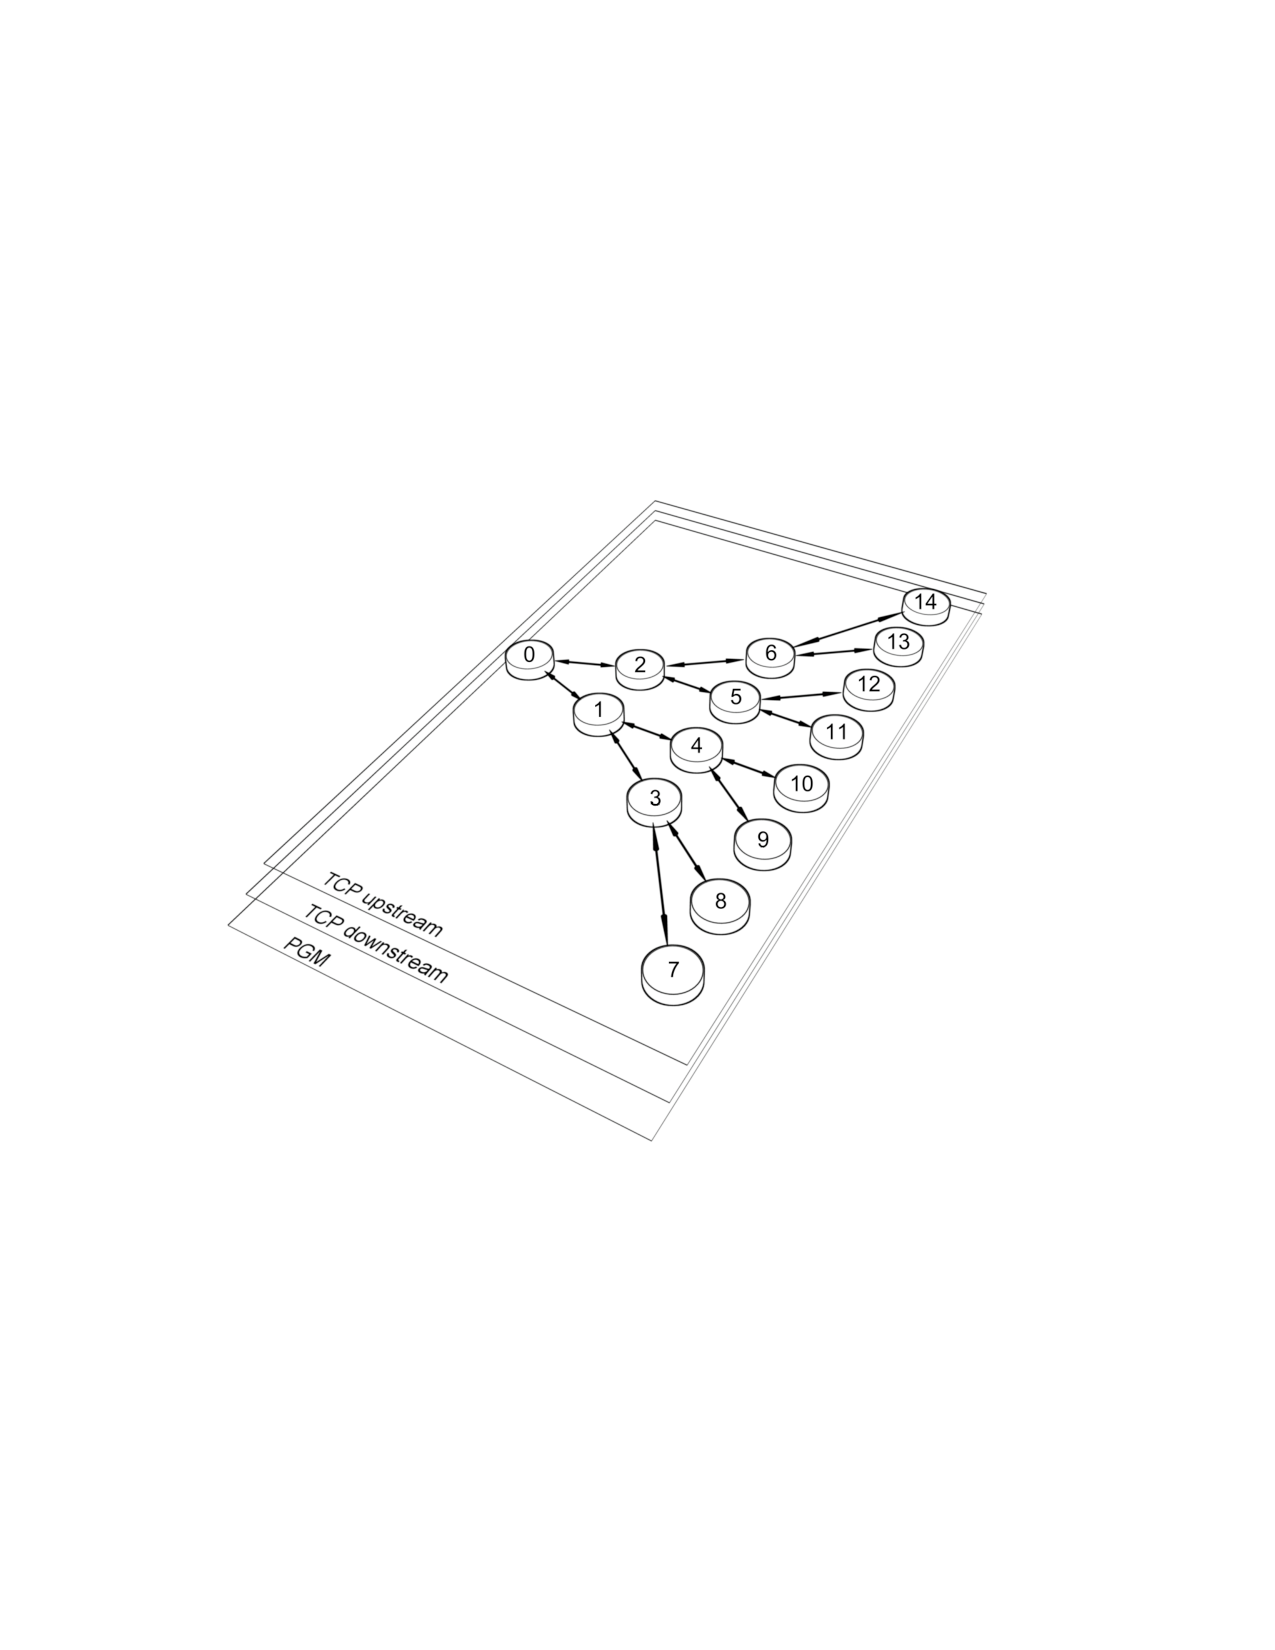
\includegraphics[trim=5.0cm 8.0cm 5.0cm 8.0cm,scale=0.40]{B_Tree_4Layer_BW}
\vspace{-.3cm}
\caption{A comms session} 
\vspace{-.5cm}
\label{fig:commswireup}
\end{figure}

We have built a primitive prototype of the \flux\ communications framework
using \zMQ~\cite{ZMQGuide} which we can launch within a
Slurm~\cite{Jette02slurm} job.
\zMQ\ provides the ability to manipulate opaque,
multipart messages, and carry them across various transports, including
TCP and Pragmatic General Multicast (PGM)~\cite{rfc3208}
using a socket-like API.
\zMQ\ provides abstractions that ease implementation of common
messaging patterns including {\em request-reply}, {\em publish-subscribe},
and {\em push-pull}.
\zMQ\ can be used to build applications or custom message brokers.


Our prototype consists of a distributed Comms Message Broker (CMB)
daemon that runs on each node of a comms session, interconnected using
three persistent overlay network planes:
a PGM {\em publish-subscribe} bus for events; 
a TCP {\em dealer-router} (advanced {\em request-response})
tree for upstream RPCs and reductions
similar to those enabled by MRNet~\cite{mrnet}; and
a secondary TCP {\em dealer-router} tree for downstream RPCs.

%consists of daemons interconnected using
%three persistent overlay network planes:
%a TCP {\em dealer-router} tree for upstream RPCs and reductions,
%a TCP {\em dealer-router} tree for downstream RPCs, and
%a PGM {\em publish-subscribe} bus for events.
%Although a binary tree is pictured, the RPC planes can be launched in
%any tree shape for testing or to tune performance.
%%Flat, degenerate, {\em k}-ary for several values of {\em k}, and
%binomial have been tested.
%}

The comms session wire-up is depicted in Figure~\ref{fig:commswireup}.
Each message plane implements reliable, in-order message delivery, and
can self-heal when nodes other than the root node fail.
Although a binary tree is pictured, the RPC planes can be launched in
any tree shape for testing or to tune performance.
Security and comprehensive fault-tolerance are not yet implemented,
but are near-term design topics.

The CMB allows us to experiment with loosely coupled distributed services
while reusing the underlying message routing framework.  Various comms
services have been implemented as CMB plugins.  Plugins currently exist for
the services listed in Table~\ref{tab:cmbplugins}.
Each embodies an active topic for study and experimentation. % by the \flux\ team.

In addition to CMB plugins, external programs can communicate with the CMB
via a UNIX domain socket.  A {\tt flux} utility wraps up two dozen or so
modular subcommands used to interact with and test the CMB plugins.

\begin{table}
\centering
\vspace{-.5cm}
\caption{Prototyped CMB plugins}
% implement basic building blocks for \flux\ and
%potentially other applications.  These are the plugins we have prototyped
%thus far, representing a wide range of design maturity.  Each embodies an
%active topic for study and experimentation by the \flux\ team.}
\begin{tabular}{|l|p{9cm}|}\hline
\textbf{Plugin} & \textbf{Description} \\
\hline
heartbeat & A periodic heartbeat event multicast across the comms
	session synchronizes background activity to reduce scheduling jitter.\\
\hline
live & Each tree node receives heartbeat-synchronized {\em hello}
	messages from its children.  After a configurable number of missed
	messages, a liveness event is issued for a dead child.\\
\hline
log & Log messages are reduced and filtered before being placed in
	a log file at the session root.  A circular debug buffer
	provides log context in response to a fault event.\\
\hline
mon & Lua scripts stored in the KVS activate heartbeat-synchronized sampling.
	Samples are reduced and stored in the KVS.\\
\hline
group & \flux\ groups define and manage collection of processes that can
	participate in collective operations.\\  
\hline
barrier & Collective barriers provide synchronization across \flux\ groups. \\
\hline
kvs & A distributed key-value store provides a scalable scratchpad
	for \flux\ and other tools operating within the comms session.\\
\hline
wrexec & Remote processes can be launched in bulk, monitored,
	receive signals, and have standard I/O captured in the KVS.\\
\hline
resrc & Resources are enumerated in the KVS and allocated
	when the scheduler runs a lightweight job. \\
\hline
sched & Lightweight job requests are queued in the KVS, assigned
	resources, and launched. \\
\hline
\end{tabular}
\label{tab:cmbplugins}
\vspace{-.5cm}
\end{table}


All CMB messages have a uniform multi-part message format consisting of
a {\em tag frame} and a {\em JSON~\cite{rfc4627} frame}.  The tag frame identifies the
message recipient using a hierarchical name space.  For example a message
sent to the tag {\em kvs.put} is routed to the {\em kvs} plugin, and internally
to its handler for {\em put}.  The tag frame format is identical to
\zMQ's {\em publish-subscribe} topic string format, thus CMB messages
have the same format on all three overlay networks.
The message payload is contained in the free-form JSON frame.

Most requests are routed via the upstream request overlay network
and utilize the \zMQ\ {\em dealer-router} pattern's built-in source routing
scheme for returning optional replies to the sender over the same network.
Requests are routed to the first plugin encountered in the tree that claims
the tag, or are negatively acknowledged at the root.  This enables plugins
to be loaded at a variable tree depth to tune its level of distribution
or conserve node resources for application workloads toward the leaves.
Reductions are simply requests that are aggregated and retransmitted between
instances of a plugin, traversing upstream.

Explicit rank-addressing is available for requests that must target a
specific CMB instance by rank.  The rank is prepended to the tag frame,
and routing tables are consulted at each hop to determine which overlay
to use to reach the destination.  If the downstream overlay is selected,
the routing table entry determines which branch of the tree to use.
In this manner an RPC can take place between any two ranks in the session.

As our designs and prototypes for basic \flux\ building blocks evolve,
the CMB evolves to provide necessary services.  For example, the CMB API
now has both C and Lua~\cite{LuaBook}  bindings and a custom event reactor interface in
response to the experience of meeting a recent milestone to launch an
MPI job internally and co-locate a distributed debugger.  Some of the building
blocks built on CMB services, such as the key-value store plugin described
in the next section, are independently undergoing design iteration.
We expect to continue evolving the CMB prototype for several more months until
our design has reached stability and we build a production-level \flux\ 
communication framework.

\subsection{Distributed Key-Value Store}

Key-Value Stores (KVS) have become ubiquitous building blocks in large-scale
internet services but have been underutilized in high performance
computing~\cite{Wang:2013:USE:2503210.2503239}.
We determined that a KVS would be a
useful building block for our new system and prototyped several designs.
Early \flux\ KVS's were based on Redis~\cite{Redis} and Twitter's
twemproxy~\cite{Twemproxy} for sharding and were used mainly to implement
PMI~\cite{PMI2} under MPI.  More recently our KVS has been employed 
in addition for configuration, monitoring, resource descriptions, and
standard I/O streams, and has been rewritten from scratch to meet these
new demands and obtain the most benefit from our persistent CMB overlay
networks.

Our current prototype stores JSON values under a hierarchical key space
with a single master node and multiple caching slaves.  The weak consistency
of our slave caches has the following properties, using Vogels'
taxonomy~\cite{Vogels:2009:EC:1435417.1435432}:
\begin{itemize}
\item{{\em causal consistency}:  If process A communicates with process B
that it has updated a data item (passing a {\em store version} in that
message), a subsequent access by process B will return the updated value.}
\item{{\em read-your-writes consistency}:  A process having updated a
data item, never accesses an older value.}
\item{{\em monotonic read consistency}:  If a process has seen a particular
value for an object, any subsequent accesses will never return previous values.}
\end{itemize}

We achieve these properties with a simple design based on hash trees
and content-addressable storage, borrowing ideas from
ZFS~\cite{Bonwick03thezettabyte}, git~\cite{Chacon:2009:PG:1618548}, and
Venti~\cite{Quinlan:2002:VNA:645371.651321}.
JSON objects are placed in a content-addressable
{\em object store}, hashed by their SHA1 digests.
Hierarchical key names are broken up into path components that reference
directories.
A directory is a table of names versus SHA1 object store references,
which is itself placed in the store.  An external root directory SHA1
reference points to the root directory.
For example, if the SHA1 root reference is {\tt 1c002dd...}, and we have
stored {\tt a.b.c = 42} in the KVS, we would look it up as follows:
\begin{enumerate}
\item{load root directory from {\tt 1c002dd...}, find {\tt a} is at
{\tt 3f2243ef...}.}
\item{load {\tt a} from {\tt 3f2243ef...}, find {\tt b} is at
{\tt 023e9b2d...}.}
\item{load {\tt b} from {\tt 023e9b2d...}, find {\tt c} is at
{\tt 7ff234a8...}.}
\item{load {\tt c} from {\tt 7ff234a8...}, and return it (42).}
\end{enumerate}

An important property of this structure is that any update results
in a new SHA1 root reference.  For example if we update {\tt a.b.c = 43}, we:
\begin{enumerate}
\item{store 43 to {\tt 62302aff...}.}
\item{update {\tt b} to associate {\tt c} with {\tt 62302aff...}, and store {\tt b} to {\tt 8fe9b2c3...}.}
\item{update {\tt a} to associate {\tt b} with {\tt 8fe9b2c3...}, and store {\tt a} to {\tt aacc76b4...}.}
\item{update root to associate {\tt a} with {\tt aacc76b4...}, and store root to {\tt 033fbe92...}.}
\item{the new root reference is {\tt 033fbe92}.}
\end{enumerate}

All updates are applied first on the master node at the root of the
CMB tree, which then publishes a new root reference as a CMB event.
Slaves keep consistent with the master by switching their root reference
in response to this event, so that all new lookups must begin at the
new root directory.  Objects missing from the slave object cache during
a lookup are faulted in from their CMB tree parent, recursing up the tree
until the request can be fulfilled.  Unused slave object cache entries are
expired after a period of disuse to save memory.

The CMB event overlay network guarantees ordered delivery, which gives
us monotonic read consistency for free.  We achieve read-your-writes
consistency by returning the new root reference in response to a commit
request and applying it before returning to the caller.  We avoid
racing with the event update and potentially breaking monotonic read
consistency by versioning the root references and never running it
backwards.  We achieve causal consistency by allowing this version number
to be read after an update, and by providing another call to wait for this
root version or greater on another node before accessing the value.

The KVS API includes classes of functions for putting, commiting, and
getting KVS objects.  We refer to these classes as
{\em producer}, {\em synchronization}, and {\em consumer} respectively
in the results section.

{\em kvs\_put (key, val)}
writes {\em val} to the object store asynchronously in a write-back
mode through the tree of slave caches.
The ({\em key, SHA1}) tuple is cached locally pending commit.

{\em kvs\_commit ()} synchronously flushes ({\em key, SHA1}) tuples
and any still-dirty objects to the master.  On the master, it then
processes the set of tuples, creating new directory objects as described
above, finally arriving at a new root SHA1.  It then updates the 
root reference session-wide with a multicast event.
Since both new and old objects coexist in the caches, the switch from old
to new root is atomic.
There is also a {\em kvs\_fence} call which commits for a group of
processes collectively, through the internal use of a collective barrier
and slight modification to the commit logic on the master.

{\em kvs\_get (key)} recursively looks up the key starting with the
current root reference as described above, faults in any missing objects
through the tree of slave caches, and returns the terminal object.
{\em kvs\_watch (key, callback)} is a get variant which registers a
callback to be triggered whenever the value of {\em key} changes.
It accomplishes this by internally by performing a get on the watched
value in response to each root update, comparing the new
and old values, and calling the callback if they are different.
Due to the internal hash tree organization, a watched directory changes
if keys under it at any path depth change.

The theoretical performance of our KVS prototype should be influenced by
the following aspects of the design:
\begin{itemize}
\item{Slave caches are arranged hierarchically so that the effect of a
cache miss across a large number of processes is mitigated by the tree
fanout.}
\item{The act of storing an object redundantly in the object store
is squashed at the first node in the CMB tree that has the object
in cache, thus identical values and directories are reduced automatically.}
\item{Updates arriving in rapid succession (within 1 msec currently) are
coalesced into a single update to avoid excessive intermediate object
versions and cache invalidations.}
\item{A {\em collective fence} operation is provided, inspired by PMIv2,
which allows updates from many processes to be coalesced into one.}
\item{The root directory object is sent along with its SHA1 reference when the
new root is published, due to the high probability of needing to fault it in.}
\item{Values amounting to an encoded JSON size less than the size of a base64
representation of its SHA1 digest are stored directly in their directory.}
\end{itemize}
Practical performance results are presented in the results section.

Work on the KVS prototype is ongoing, and our prototype still lacks some
important features that will be needed in the production version,
including the ability to make its contents persistent beyond the
life of a comms session,
tolerance of a fault of the KVS master,
and sharding.

%\subsection{Lightweight Job (LWJ)}
CMB and KVS are the scalable building blocks not only for our run-time services 
but also other key run-time software such as parallel programming models, 
tools, and middleware. These programs commonly employ distributed processes and need a 
flexible and concise mechanism to relate their processes to underlying resources 
(e.g., containing certain processes to a set of resources) as well as relate 
them to other processes. 

The traditional approach models those processes as
a set of compute steps---e.g., job steps. However, this model 
is MPI-centric and too static to support emerging types
of run-time patterns arising from dynamic workload, tools, and middleware.
Thus, we introduce a more flexible concept called the lightweight job (LWJ).
A LWJ is a group
of processes with a distinct function that has its own resource confinement. 
For example, all of the parallel
processes of an MPI application may form a single compute LWJ; all of the distributed processes
of a parallel debugger program may form a tool LWJ that should be logically separate from the
compute LWJ; further, the compute LWJ may dynamically refine itself into several 
sub groups to serve independent power-capping functions to different subsets of its processes.
We currently use the KVS to organize LWJ information hierachically.

\section{Results}
\label{sec:results}
One of the most important initial goals of \flux\ is to gain
a fundamental understanding of key design challenges pertaining
to our conceptual models.
In the context of \flux's run-time system, the scalability
and productivity
challenges---as described in Section~\ref{sect:challenges}---are especially
relevant and crucial. 
%Clearly, we  must provide a wide range
%of run-time elements such as parallel programming models,
%tools and middleware with performance, scalability, easy integration
%and interoperability.
Thus, this section evaluates our prototype's performance
and scalability characteristics as well as its ability
to support various productivity software programs. 

One of the most important initial goals of \flux\ is to gain
a fundamental understanding of key design challenges pertaining
to the major shift in the new RM conceptual model.
In the context of \flux's run-time system, the scalability
and productivity
challenges---as described in Section~\ref{sect:challenges}---are especially
relevant and crucial. Clearly, we  must provide a wide range
of run-time elements such as parallel programming models,
tools and middleware with performance, scalability, easy integration
and interoperability.
This section evaluates our prototype's performance
and scalability characteristics as well as its ability
to support various HPC run-time elements.


\subsection{KVS Access Patterns (KAP) Tester}
To examine the performance of \flux's run-time system,
we developed a tester called KVS Access Patterns (KAP).
\begin{figure}
  \centering
  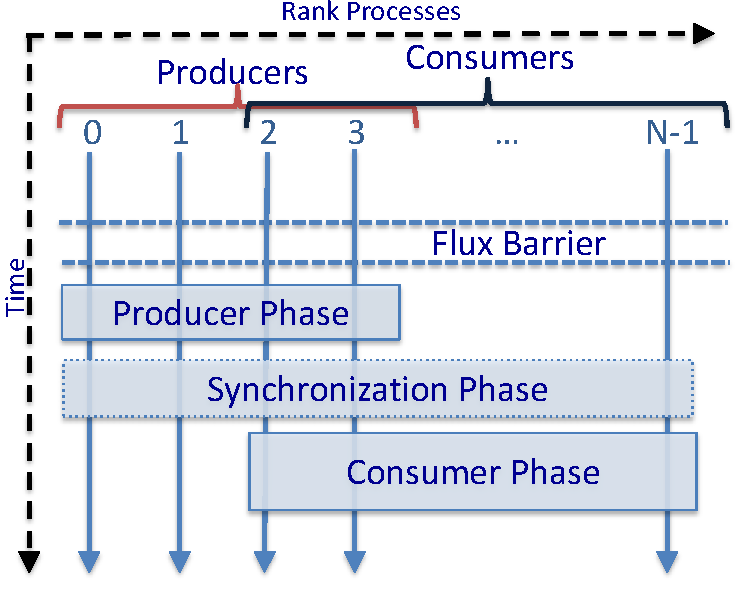
\includegraphics[scale=0.45]{kaptester}
  \caption{Main phases of KAP tester}
  \label{fig:kap}
\end{figure}
KAP models KVS access patterns through various interactions
between KVS writers and readers. Writers are called producers;
readers consumers.
In essence, KAP allows a configurable number of producer processes
to write key-value objects into our KVS 
and a configurable number of consumers to read these
objects after ensuring the consistent KVS state.

In addition to producer and/or consumer counts,
KAP provides a range of parameters that can affect performance.
Among them include the value size (of key-value objects),
the number of objects to put,
the number of objects to read, objects access 
patterns (through different striding), and
synchronization primitives used for consistency.

Figure~\ref{fig:kap} shows the three main phases of KAP.
Right after tester processes are launched into a set of nodes
in which a CMB session had been established,
they are assigned to ranks such that consecutive rank
processes are distributed to consecutive nodes.
Then, the rank processes determine their roles based
on the command line arguments and issue a named barrier
that \flux\ provides to begin to play their roles
simultaneously.

Next, each producer calls the specified number of
{\tt kvs\_put}s of an object of the specified value size.
For each call, the producers use unique keys, but
the values can be configured to be either unique
or redundant.
Once this producer phase completes, all of the producers and consumers
participate in a consistency protocol that uses
\flux's synchronization primitives such as the collective
fence---i.e., the {\tt kvs\_fence} function.
Finally, during the consumer phase, consumers read
these key-value objects by calling {\tt kvs\_get}s.
KAP provides options to emulate various read access
patterns.


\subsection{Experimental Setup}
We run all of our experiments on two Linux clusters installed at LLNL,
named Zin and Cab.
Each compute node of these clusters has 2 sockets and 32 GB of RAM.
Each socket is populated with an 8-core 2.6 GHz Intel
Xeon E5-2670 processor, resulting in 16 cores per node.
Zin consists of 2,916 compute nodes totaling 46,656 cores;
Cab is a smaller system with the same node type,
consisting of 1,296 compute nodes with a total of 20,736 cores.
Nodes are connected by a Qlogic Infiniband QDR interconnect.
The largest allocation allowed in normal batch mode
is 258 nodes on Cab and 512 on Zin.

We run KAP with varying arguments to its parameters
in batch mode and collect various 
performance metrics. 
Because the exploration
space is huge, however, we limit our experiments with
only a subset of the parameter set and of sampling points.

Specifically, we run our KAP tests at 64, 128, 256 and 512
compute nodes, and always fully populate each node with
16 processes, each acting as consumer or producer or
both. We vary the consumer or producer count
while fixing the other at the total number of cores.
We also vary the value size 
from 8 Bytes to 32 Kilobytes in the powers of 8,
and the key-value object access count of each consumer
from 1 to the total process count.

Further, we evaluate the performance impact 
of how key-value objects are organized 
in KVS by either storing all of the objects into a single KVS directory
or distributing them into multiple directories---i.e.,
128 objects per KVS directory.
Finally, we study the performance implications of 
redundancy in values by either configuring producers to generate
unique or redundant values across them.

For simplicity, we configure the topology of CMB only as 
the binary tree and and use \flux's collective fence 
as our only mechanism to enforce consistency.

\subsection{Performance Results and Analysis}
\label{results}
Of tens of thousands of our sampling runs, we find that the fully populated
cases---i.e. both producer and consumer counts become equal to the total
process count---are most revealing. In particular, we carefully analyze 
the maximum latency of each of the main phases of KAP for these cases 
because this metric represents the critical path of the performance of
many HPC services. For example, distributed 
HPC software would use KVS operations in a coordinated fashion to exchange 
connection information among processes during its bootstrapping 
phase~\cite{LIBI,PMI2}. Unless {\em all} 
of the distributed processes complete their
KVS operations, their communication fabric cannot be established. 

\begin{wrapfigure}{l}{80mm} 
  \centering
  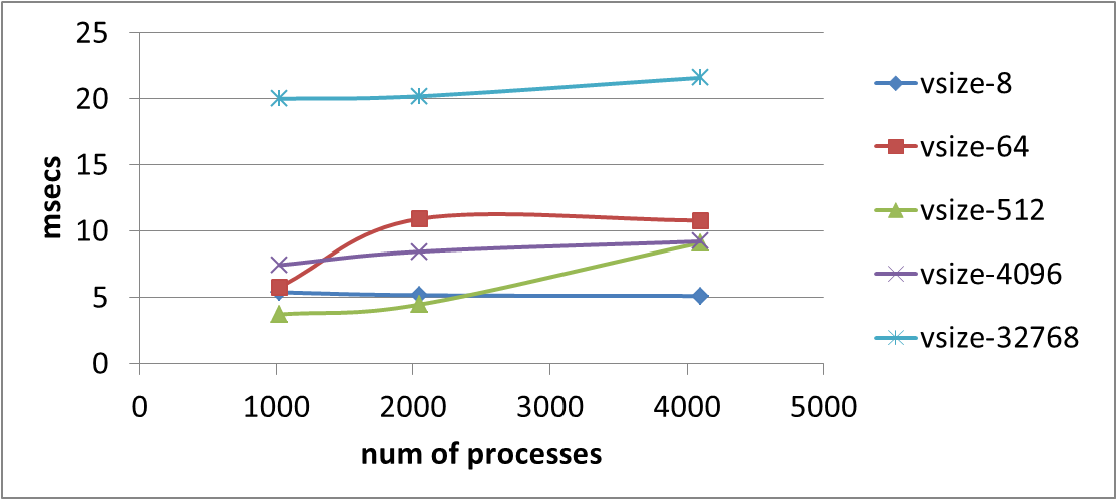
\includegraphics[scale=0.40]{producer}
  \caption{Max latency of producer phase}
  \vspace{-.5cm}	
  \label{fig:prod}
\end{wrapfigure}

Figure~\ref{fig:prod} shows the maximum latency of the producer phase
for these cases. Essentially, these lines indicate how well {\tt kvs\_put}
scales as we increase the number of producers. Each line represents
different value sizes---e.g., vsize-8 refers to value size being
8 Bytes. As shown in this graph, the {\tt kvs\_put} simply performs and
scales well. This matches our expectations because the key-value objects
are locally cached at {\tt kvs\_put} time and pushed to the
server at the next consistency event. 

\ifcomments
\marginpar{\tiny DA: I will add data from 8K if I get it on Zin in time.}

\begin{figure}[ht]
\centering
\begin{subfigure}[With unique values]{
  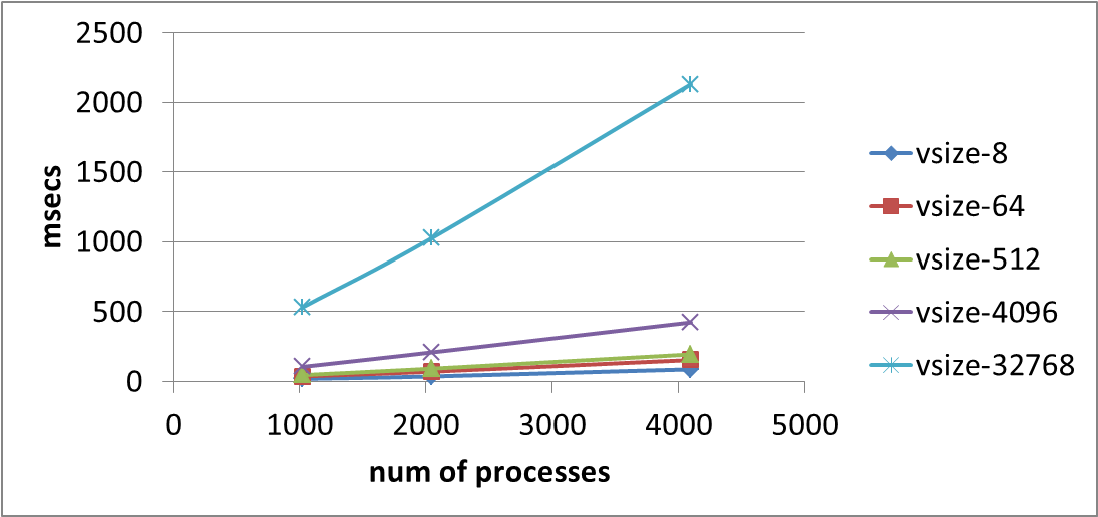
\includegraphics[width=.75\linewidth]{sync}
  \label{fig:sync:noredund}
}%
\end{subfigure}
\begin{subfigure}[With redundant values]{
  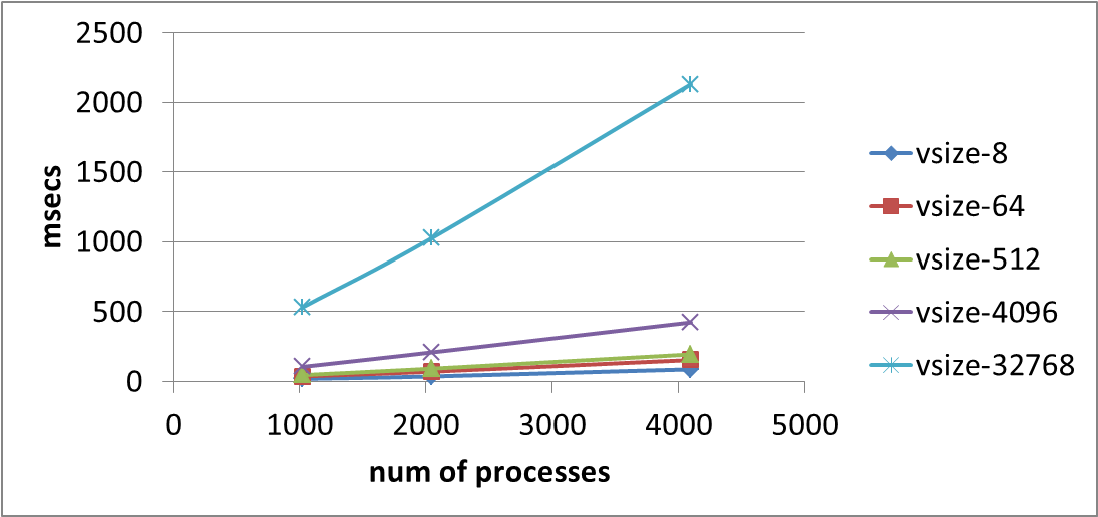
\includegraphics[width=.75\linewidth]{sync}
  \label{fig:sync:redund}
}%
\end{subfigure}
\caption{Max latency of synchronization phase}
\label{fig:sync}
\end{figure}


Moving onto the synchronization phase, Fig.~\ref{fig:sync} shows 
how well {\tt kvs\_fence} scales during this phase,
as we increase the number of producers. 
As with the producer latency,
each line represents different value sizes.  
The most revealing observation is that 
fence scalabilty appears to depend on the level of
redundancy in key-value objects that had previously 
been put in. Figure~\ref{fig:sync:redund} 
shows the maximum latency of the synchronization phase
when redundant values are used. It scales
far better than Fig.~\ref{fig:sync:noredund}
where there is zero redundancy in values. 
We theorize that in the former case, fence performs linearly with respect to the number of
producers because these unique values are being {\em concatenated} while
being sent up the tree. It performs logarithmically for the latter case
because redundant values are being {\em reduced} while being sent 
up the tree. %%(MENSION R^2 here?)

\marginpar{\tiny DA: I am speculating a bit for redundant case; my job on cab will confirm or deny this.}

\begin{figure}[ht]
\centering
\begin{subfigure}[With single-directory layout]{
  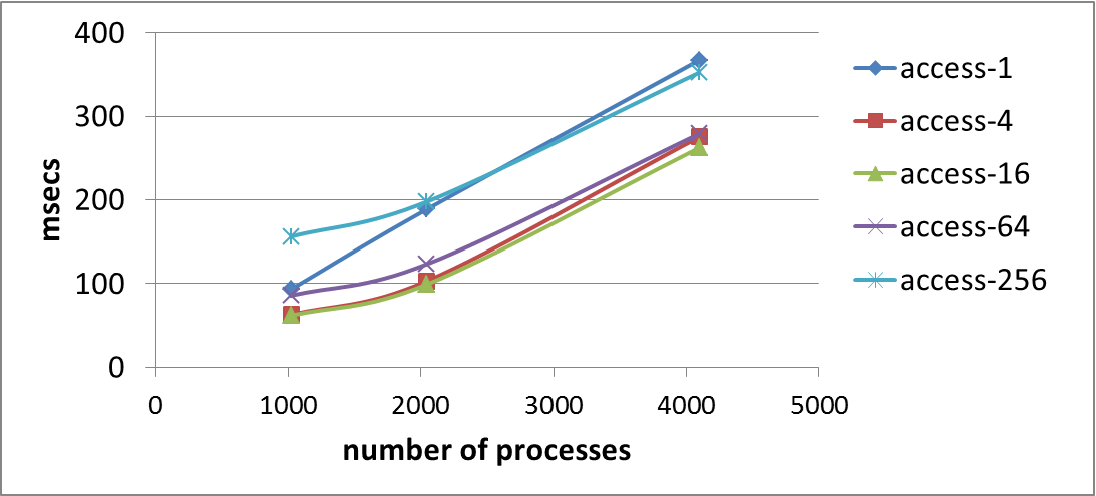
\includegraphics[width=.75\linewidth]{consumer-1-dir}
  \label{fig:cons:dir}
}%
\end{subfigure}
\begin{subfigure}[Improvements with multiple directories]{
  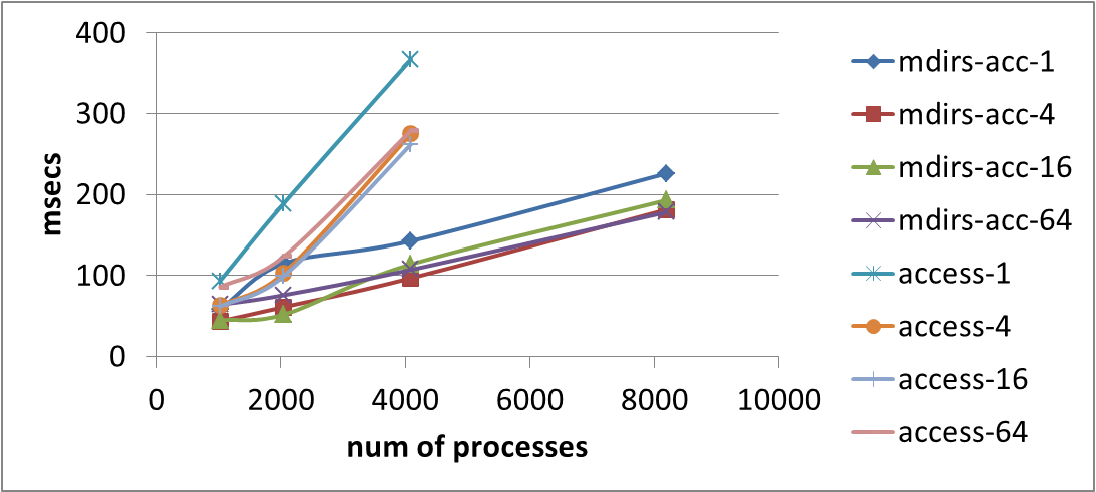
\includegraphics[width=.75\linewidth]{consumer-dist-dir}
  \label{fig:cons:dirs}
}%
\end{subfigure}
\caption{Max latency of consumer phase (value size: 8 Bytes)}
\vspace{-.5cm}
\label{fig:consumer}
\end{figure}

Figure~\ref{fig:consumer} shows the maximum latency of the consumer
phase with respect to various parameter settings. 
The lines generally suggest how well {\tt kvs\_get}
scales, as we increase the number of consumers. Each line represents
the latency when each consumer reads different numbers of 
key-value objects---e.g., access-4 refers to read 4 distinct key-value 
objects. While these figures show only the performance of reading
objects with 8-Byte value, we observe that the general 
scalability trends are similar at different value sizes.

Figure~\ref{fig:cons:dir} shows the maximum latency of {\tt kvs\_get}
when the target key-value objects are all stored in a single
KVS directory. The latency is quite high and also increases
linearly, as we increase the number of consumers. 
It appears that the poor performance and scaling behavior 
are attributed to KVS replication granularity and 
the fact that the objects are stored in a single directory.

When {\tt kvs\_get} cannot be satisfied by the local KVS replica,
our system ensures that the entire directory where
the requested object resides is replicated on
all of the ancestor CMB daemons that are along the direct path 
to the root. With our access pattern where all objects
are read collectively by consumers, this means the latency is 
$log_2(C) \times T_{replicate}(G)$, where C is the consumer count, and G is the 
total amount of data in the master KVS server.
Thus, the max latency increase for every doubling of consumers is 
$\frac{log_2(2C) \times T_{replicate}(2G)}{log_2(C) \times T_{replicate}(G)}$.
Generally, this would approach 2, 
as we continue to increase the number of consumers,
and our data match with this model.

We can improve this behavior by storing objects across multiple
directories. With such an organization, the size of replicas 
would decrease as we go down the CMB tree. This is of course only when
each consumer reads only a small fraction of data. In another
word, if each consumer read all of the data in KVS, the latency
would be same as the single directory case. 
Figure~\ref{fig:cons:dir} shows the improvements 
when we spread objects into multiple directories by
keeping the number of objects per directory constant: 128.
Label {\tt mdir-acc-k} refers to the same access pattern as {\tt access-k} 
except the accessing objects are stored across multiple directories.


For the case where the size of replicas 
decreases as a function of tree levels, 
we can model the latency as a geometric series. For example, at tree height being $h$,
the latency would be 
$T_{replicate}(G) + T_{replicate}(\frac{G}{2}) + T_{replicate}(\frac{G}{4}) + ... + T_{replicate}(\frac{G}{2^h})$, 
where each term represents the latency of replication per level.
This would approach $2T_{replicate}(G)$. Thus, its improvement over the single
directory scheme is: $\frac{log_2(C) \times T_{replicate}(G)}{2 T_{replicate}(G)}$.
Roughly speaking, the improvements would be on the order of 
$\frac{1}{2}log_2(C)$. The improvements would be linearly 
greater as we increase the scale and our measurements agree with this. 

While significant, we note that a smarter KVS data layout scheme alone
can still fall short of reaching extreme scale. Our model tells us that the latency
will grow linearly when $G$ grows with the scale. 
Say, $G$ doubles every time you double the number of consumers, our geometric series
model predicts the latency will also double:
$\frac{2T_{replicate}(2G)}{2T_{replicate(G)}}$ becomes 
on the order of 2. With the current scheme, the only true way to gain logarithmic
scaling is when $G$ stays constant regardless of scale. 
In a later section, we will discuss some of our plans 
to exploit the understanding we gain from the evaluation. 




%\subsection{Case study: Easy Integration of Tools and Middleware}

TBD

\section{Related Work}
\flux seeks to change the paradigm in which 
how large HPC centers should manage, model, schedule, and
allocate resources. 
A strong body of research exists in each of these areas 
including production solutions such as SLURM~\cite{Jette02slurm}, 
LSF~\cite{LSF}, Moab~\cite{MOAB}, 
PBS Pro~\cite{PSBPro}, LoadLeveler~\cite{LL}
and Condor~\cite{Litzkow88}.
To the best of our knowledge, \flux is a novel open-source 
effort that tackles emerging HPC resource management challenges 
by raising the RJMS's purview to the entire center 
under one common software framework. 

In other areas such as cloud or grid computing, the need 
for exploting scheduler parallelism including two-level 
scheduling also recently emerged. 
Google's Omega~\cite{Omega} exploits 
a parallel scheduler architecture whereby multiple
schedulers concurrently access the shared resource state
with an optimistic concurrency model. Efforts
such as Apache Mesos~\cite{Mesos} and many emerging
grid schedulers~\cite{MultilevelGrid,Oar} 
take advantage of two-level scheduling strategies.
However, these approaches are neither optimized for HPC workloads 
and nor well suited for large HPC centers. 
Scales of a large HPC center demand a deeper 
and dynamic resource management and scheduler hierachy 
with an ability to impose various policies and
constraints at various levels in this hierachy.

HPC trends increasingly motivate scalable KVS implementations 
like ours. Wang et al. proposed a distributed KVS 
as the basis for HPC tools and services to encapsulate
complexity of distributed services~\cite{Wang:2013:USE:2503210.2503239}.
%
%, thereby simplifying the
%tools and services~\cite{Wang:2013:USE:2503210.2503239}.
They further evaluate replacing the centralized controller in
Slurm~\cite{Jette02slurm} with a distributed controller~\cite{Slurmpp}
built on ZHT~\cite{Li:2013:ZLR:2510661.2511401}.
While existing KVS work takes an incremental approach of improving 
scalability of a traditional RJMS paradigm with new scalable services,
ours are built specifically to support the new paradigm. 

We also evaluated Redis~\cite{Redis} and twemproxy~\cite{Twemproxy}
as part of our early KVS investigations.
%In particular, Redis cluster~\cite{RedisClusterTut,RedisClusterSpec} 
%includes many desired properties such as 
%sharding, re-sharding, replication, and failover.
%However, their design points are not optimized
for HPC workloads which often feature synchrony and coordination. 
Our consistency model and mechanisms such as the collective fence 
specifically optimized for HPC.


%There is no proxy; clients connect directly to the server
%for a particular shard.  Redis-cluster's asynchronous replication
%results in the possibility of losing writes that occur during failover.
%
Finally, much research exists in the area of tree-based overlay network (TBON). 
They include MRNet~\cite{mrnet} and COBO~\cite{launchmon}, and 
%In particular, MRNet is a reusable designed to be embedded 
%in large scale HPC tools such as STAT~\cite{STAT}. 
%%They have explored
%{\em state compensation}~\cite{conf/ipps/ArnoldM10}
%as a mechanism for fault tolerance in TBONs that perform data aggregation.
CMB can be considered to be a TBON. But unlike user-level
TBONs, ours must support system-level activities, and this 
requires us to answer distinct research topics
such as support for multiple user-level networks (which actually
include other user-level overlay networks), security, low noise 
and fault tolerance. 


\section{Conclusion}
Large HPC centers are increasingly facing 
multifaceted resource management challenges
that if not properly met, will result 
in significant losses.  
\flux\ is our response to these challenges
so as to improve operational efficiency 
and user productivity by changing 
the fundamental way in which large
centers are managed.
Our run-time infrastructure such as CMB and KVS
is a significant first step to this rather long
journey.

We have validated key aspects of these
components to guide our future efforts systematically. 
Our study suggests that our run-time 
infrastructure is most scalable when information 
exchange patterns themselves are also scalable.
And this suggests two significant directions. 
For one, we must carefully design the data exchange patterns
among distributed components of run-time elements. 
To achieve extreme scalability, each component 
must avoid accessing a global view.
Secondly, we must also continue to push the 
scalability envelope of our infrastructure. 
For the latter, we will soon investigate a way to 
shard KVS masters into multiple nodes
and to distribute access patterns to further improve scalability.

Besides scalability, we must also address KVS persistency.
Specifically, we plan to explore a scheme
thereby putting on-disk cache behind the KVS master,
and then temporally expire the master's cache.
In fact, we will investigate ways to link
this scheme to the sharding scheme such a way
that a single on-disk cache can service the value
objects to all of the KVS masters.

There are other deficiencies we must address as well.
These include network security and
comprehensive fault tolerance. 
As we continue to implement these building blocks 
to further our framework, we will be evaluating 
whether the framework can meet our goal for \flux's 
flexibility, scalability, and extensibility. 
Ultimately, it is our hope that \flux\ will 
enable developers at the operating system and
run-time levels to leverage the RM data stores and services in
unprecedented ways, and that it will position HPC centers to cope
with diverse, extreme-scale resources.


%Interestingly, if KVS persistence were implemented using an on-disk
%object directory structured like the git's~\cite{Chacon:2009:PG:1618548},
%which uses SHA1 digests as file names, it could be shared across multiple
%masters using a network file system like NFS with close-to-open cache
%coherency, since file names will always refer to the same content and
%published references could be guaranteed coherent.
%Such a scheme could be used to build a clustered KVS master with each
%node in the cluster servicing disjoint shards of the key space but
%sharing a common object store.





%The original \flux\ design described a job and hence a comms session
%as having an owner with the ability to control what other users could
%execute within the job, including the ability to launch new jobs and
%launch LWJ's within the current job.  In addition, the job would launch
%work in lightweight, virtualized containers that prevented LWJs from
%exceeding their resource allocation.  Finally, a job could span any set
%of resources across a data center, meaning comms session overlays must
%be capable of spanning multiple, possibly disjoint IP networks.
%These features will require the \flux\ communications framework to
%support message intergrity and privacy so that users cannot interfere
%with one another or attain inappropriate privileges, and to integrate with
%enterprise authentication services such as Kerberos.
%

%The current KVS object cache is stored in memory.
%On slave caches, objects are expired after a period of disuse.
%On the master, however, objects must remain in memory forever.
%Over time, the cache will become filled with old values that may never
%be used again.  One solution to this problem is to add a level of
%on-disk cache behind the master, and then temporally expire the master's
%cache in a manner similar to the slave caches.  This would allow data from
%the KVS belonging to a job to be {\em reaped} at job termination and
%incorporated in some reduced form into the KVS of the parent job.
%
%Interestingly, if KVS persistence were implemented using an on-disk
%object directory structured like the git's~\cite{Chacon:2009:PG:1618548},
%which uses SHA1 digests as file names, it could be shared across multiple
%masters using a network file system like NFS with close-to-open cache
%coherency, since file names will always refer to the same content and
%published references could be guaranteed coherent.
%Such a scheme could be used to build a clustered KVS master with each
%node in the cluster servicing disjoint shards of the key space but
%sharing a common object store.
%
%There are other deficiencies we must address as well.
%These include network security, comprehensive fault tolerance,
%KVS persistance, and KVS clustering.

%The \flux\ CMB detects non-responsive nodes, evicts them from
%the session, and alters its topology to work around them.
%There is not a comprehensive strategy for ensuring that all in-flight
%RPC's complete or are restarted across one of these fail-over events,
%and that state from the evicted node is recoverable.
%


%\section {Acknowledgments}
The authors acknowledge the contributions of Matthieu Hautreux
of Commissariat a l'Energie Atomique et aux Energies Alternatives
and Jon Bringhurst of Los Alamos National Laboratory, who reviewed
and provided substantial and insightful feedback on the unpublished
\flux\ functional design document, and in subsequent discussions.
\ifcomments
\marginpar{\tiny BS: Or something like that}
\fi

This article has been authored by Lawrence Livermore National Security, LLC
under Contract No. DE-AC52-07NA27344 with the U.S. Department of
Energy. Accordingly, the United States Government retains and the publisher,
by accepting the article for publication, acknowledges that the United States
Government retains a non-exclusive, paid-up, irrevocable, world-wide license
to publish or reproduce the published form of this article or allow others to
do so, for United States Government purposes. (LLNL-CONF-xxxxxx).


\bibliographystyle{IEEEtran}
\bibliography{../bib/project.bib,../bib/rfc.bib}

\end{document}
